\documentclass[12pt]{article}
\usepackage{geometry}
\usepackage[utf8]{inputenc}
\usepackage[spanish]{babel}
%\usepackage[square,numbers, sort]{natbib}
\usepackage[colorlinks, citecolor = blue, linkcolor = blue]{hyperref}
\usepackage[dvipsnames]{xcolor}
\usepackage{enumitem}
\usepackage{sectsty}
\usepackage{multicol}
\usepackage{fancyvrb}
\usepackage{amsmath}
\usepackage{graphicx}

\usepackage[backend=bibtex, style=chem-acs, natbib=true]{biblatex}

\DeclareCiteCommand{\citeauthor}%
{\boolfalse{citetracker}%
	\boolfalse{pagetracker}%
	\usebibmacro{prenote}}
{\ifciteindex
	{\indexnames{labelname}}
	{}%
	\printtext[bibhyperref]{\printnames{labelname}}}
{\multicitedelim}
{\usebibmacro{postnote}}
\addbibresource{bibliography.bib} % The filename of the bibliography

%\chapterfont{\color{blue}}  % sets colour of chapters
\sectionfont{\color{blue}}
\subsectionfont{\color{blue}}
\subsubsectionfont{\color{blue}}
\paragraphfont{\color{blue}}


\title{\color{blue} \scshape{GAPDH\\ enzima recombinante}}
\author{Juan Barbosa - 201325901}

\newcommand{\enzima}{\textbf{GAPDH}}

\begin{document}
	\maketitle
%	\dominitoc
	\begin{multicols}{2}
		\footnotesize
		\tableofcontents
	\end{multicols}
	\rule{15cm}{0.4pt}

	\section{C\'omo extraer el DNA}
		Dado que la \enzima{} tiene un origen humano, la muestra de DNA ser\'ia obtenida a partir de sangre humana. Con el objetivo de preservar la muestra, hasta el momento de la extracci\'on del material gen\'etico, a la sangre se le agregar\'ia EDTA como anticoagulante, y ser\'ia conservada a 4 $^\circ$C \cite{m2011human, puregeneBook}.
		\subsection{M\'etodo de extracci\'on}
			Considerando una muestra de 300 $u$L de sangre, y usando el kit \textit{Gentra Puregene Blood Kit} para extraer el DNA, los pasos necesarios son los siguientes:
			\begin{enumerate}[label=\color{blue}\theenumi]
				\item Agregar 0.9 mL de la soluci\'on de lisis RBC (\textit{Red Blood Cells}) a un falcon
				\item Agregar 300 $\mu$L de la muestra de sangre al mismo falcon y mezclar 10 veces por inversi\'on
				\item Incubar la mezcla a 25 $^\circ$C por 1 minutos
				\item Centrifugar a 13000 rpm por 20 segundos para precipitar las c\'elulas blancas
				\item Retirar el sobrenadante dejando 10 $\mu$L en el falcon
				\item Agitar el falcon para resuspender el residuo s\'olido
				\item Agregar 300 $\mu$L de la soluci\'on de lisis celular, y agitar
				\item Agregar 1.5 $\mu$L de \textit{RNaseA Solution}, mezclar y encubar a 37 $^\circ$C por 15 minutos
				\item Agregar 0.1 mL de la soluci\'on para la precipitaci\'on de prote\'inas y agitar
				\item Centrifugar por 1 minuto a 13000 rpm
				\item Pipetear 300 $\mu$L de alcohol isoprop\'ilico a un tubo de 1.5 mL, y agregar el sobrenadante del paso anterior, y mezclar hasta observar el DNA
				\item Centrifugar por 1 minuto a 13000 rpm
				\item Descartar el sobrenadante
				\item Agregar 300 $\mu$L de etanol al 70 \% al contenedor del DNA previamente extra\'ido
				\item Centrifugar por 1 minuto a 13000 rpm
				\item Descartar el sobrenadante y secar el DNA con una corriente de aire por 5 minutos
				\item Agregar 100 $\mu$L de la soluci\'on \textit{DNA Hydratation Solution} y agitar
				\item Incubar por 5 minutos a 65 $^\circ$C para disolver el DNA
			\end{enumerate}
			
			\begin{flushright}
				Procedimiento reportado por \citeauthor{puregeneBook}
			\end{flushright}
		
		\subsection{Caracterizaci\'on}
			La determinaci\'on de la pureza del DNA extra\'ido se puede cuantificar usando espectroscop\'ia UV-Vis. Depositando una peque\~na cantidad del DNA extra\'ido en una celda de cuarzo, cuya concentraci\'on sea cercana a 20 $\mu$g/mL y midiendo el coeficiente A$_{260}$/A$_{280}$ y A$_{260}$/A$_{230}$, donde A$_\lambda$ corresponde con las absorbancias en $\lambda$ nm \cite{olson2012dna}.
			\paragraph{A$_{260}$/A$_{280}$:} Un valor cercano a 1.8 ser\'ia indicativo de un DNA puro \cite{wilfinger1997effect, green2012molecular}.
			\begin{itemize}
				\item Desviaciones positivas a este valor estar\'ian asociadas a contaminaci\'on con RNA
				\item Desviaciones negativas estar\'ian asociadas con la presencia de prote\'inas
			\end{itemize}
			\paragraph{A$_{260}$/A$_{230}$:} Los valores esperados se encuentran en el rango de 2.0 a 2.2 \cite{green2012molecular}.
			
	\section{Amplificaci\'on del gen}
		El gen que codifica para la enzima \enzima{} se encuentra en el cromosoma 12 de los seres humanos. La secuencia de nucle\'otidos se muestra a continuaci\'on y corresponde con 3859 bp \cite{NCBI}.
		\begin{Verbatim}[commandchars=\\\{\}]
GCTCTCTGCTCCTCCTGTTCGACAGTCAGCCGCATCTTCTTTTGCGTCGCCAGGTGAAGACGGGCGGAGA
GAAACCCGGGAGGCTAGGGACGGCCTGAAGGCGGCAGGGGCGGGCGCAGGCCGGATGTGTTCGCGCCGCT
GCGGGGTGGGCCCGGGCGGCCTCCGCATTGCAGGGGCGGGCGGAGGACGTGATGCGGCGCGGGCTGGGCA
TGGAGGCCTGGTGGGGGAGGGGAGGGGAGGCGTGTGTGTCGGCCGGGGCCACTAGGCGCTCACTGTTCTC
TCCCTCCGCGCAGCCGAGCCACATCGCTCAGACACCATGGGGAAGGTGAAGGTCGGAGTCAACGGGTGAG
TTCGCGGGTGGCTGGGGGGCCCTGGGCTGCGACCGCCCCCGAACCGCGTCTACGAGCCTTGCGGGCTCCG
GGTCTTTGCAGTCGTATGGGGGCAGGGTAGCTGTTCCCCGCAAGGAGAGCTCAAGGTCAGCGCTCGGACC
TGGCGGAGCCCCGCACCCAGGCTGTGGCGCCCTGTGCAGCTCCGCCCTTGCGGCGCCATCTGCCCGGAGC
CTCCTTCCCCTAGTCCCCAGAAACAGGAGGTCCCTACTCCCGCCCGAGATCCCGACCCGGACCCCTAGGT
GGGGGACGCTTTCTTTCCTTTCGCGCTCTGCGGGGTCACGTGTCGCAGAGGAGCCCCTCCCCCACGGCCT
CCGGCACCGCAGGCCCCGGGATGCTAGTGCGCAGCGGGTGCATCCCTGTCCGGATGCTGCGCCTGCGGTA
GAGCGGCCGCCATGTTGCAACCGGGAAGGAAATGAATGGGCAGCCGTTAGGAAAGCCTGCCGGTGACTAA
CCCTGCGCTCCTGCCTCGATGGGTGGAGTCGCGTGTGGCGGGGAAGTCAGGTGGAGCGAGGCTAGCTGGC
CCGATTTCTCCTCCGGGTGATGCTTTTCCTAGATTATTCTCTGGTAAATCAAAGAAGTGGGTTTATGGAG
GTCCTCTTGTGTCCCCTCCCCGCAGAGGTGTGGTGGCTGTGGCATGGTGCCAAGCCGGGAGAAGCTGAGT
CATGGGTAGTTGGAAAAGGACATTTCCACCGCAAAATGGCCCCTCTGGTGGTGGCCCCTTCCTGCAGCGC
CGGCTCACCTCACGGCCCCGCCCTTCCCCTGCCAGCCTAGCGTTGACCCGACCCCAAAGGCCAGGCTGTA
AATGTCACCGGGAGGATTGGGTGTCTGGGCGCCTCGGGGAACCTGCCCTTCTCCCCATTCCGTCTTCCGG
AAACCAGATCTCCCACCGCACCCTGGTCTGAGGTTAAATATAGCTGCTGACCTTTCTGTAGCTGGGGGCC
TGGGCTGGGGCTCTCTCCCATCCCTTCTCCCCACACACATGCACTTACCTGTGCTCCCACTCCTGATTTC
TGGAAAAGAGCTAGGAAGGACAGGCAACTTGGCAAATCAAAGCCCTGGGACTAGGGGGTTAAAATACAGC
TTCCCCTCTTCCCACCCGCCCCAGTCTCTGTCCCTTTTGTAGGAGGGACTTAGAGAAGGGGTGGGCTTGC
CCTGTCCAGTTAATTTCTGACCTTTACTCCTGCCCTTTGAGTTTGATGATGCTGAGTGTACAAGCGTTTT
CTCCCTAAAGGGTGCAGCTGAGCTAGGCAGCAGCAAGCATTCCTGGGGTGGCATAGTGGGGTGGTGAATA
CCATGTACAAAGCTTGTGCCCAGACTGTGGGTGGCAGTGCCCCACATGGCCGCTTCTCCTGGAAGGGCTT
CGTATGACTGGGGGTGTTGGGCAGCCCTGGAGCCTTCAGTTGCAGCCATGCCTTAAGCCAGGCCAGCCTG
GCAGGGAAGCTCAAGGGAGATAAAATTCAACCTCTTGGGCCCTCCTGGGGGTAAGGAGATGCTGCATTCG
CCCTCTTAATGGGGAGGTGGCCTAGGGCTGCTCACATATTCTGGAGGAGCCTCCCCTCCTCATGCCTTCT
TGCCTCTTGTCTCTTAGATTTGGTCGTATTGGGCGCCTGGTCACCAGGGCTGCTTTTAACTCTGGTAAAG
TGGATATTGTTGCCATCAATGACCCCTTCATTGACCTCAACTACATGGTGAGTGCTACATGGTGAGCCCC
AAAGCTGGTGTGGGAGGAGCCACCTGGCTGATGGGCAGCCCCTTCATACCCTCACGTATTCCCCCAGGTT
TACATGTTCCAATATGATTCCACCCATGGCAAATTCCATGGCACCGTCAAGGCTGAGAACGGGAAGCTTG
TCATCAATGGAAATCCCATCACCATCTTCCAGGAGTGAGTGGAAGACAGAATGGAAGAAATGTGCTTTGG
GGAG\textcolor{green}{GCAACTAGGATGGTGTGGCT}CCCTTGGGTATATGGTAACCTTGTGTCCCTCAATATGGTCCTGTCC
CCATCTCCCCCCCACCCCCATAGGCGAGATCCCTCCAAAATCAAGTGGGGCGATGCTGGCGCTGAGTACG
TCGTGGAGTCCACTGGCGTCTTCACCACCATGGAGAAGGCTGGGGTGAGTGCAGGAGGGCCCGCGGGAGG
GGAAGCTGACTCAGCCCTGCAAAGGCAGGACCCGGGTTCATAACTGTCTGCTTCTCTGCTGTAGGCTCAT
TTGCAGGGGGGAGCCAAAAGGGTCATCATCTCTGCCCCCTCTGCTGATGCCCCCATGTTCGTCATGGGTG
TGAACCATGAGAAGTATGACAACAGCCTCAAGATCATCAGGTGAGGAAGGCAGGGCCCGTGGAGAAGCGG
CCAGCCTGGCACCCTATGGACACGCTCCCCTGACTTGCGCCCCGCTCCCTCTTTCTTTGCAGCAATGCCT
CCTGCACCACCAACTGCTTAGCACCCCTGGCCAAGGTCATCCATGACAACTTTGGTATCGTGGAAGGACT
CATGG\textcolor{green}{TATGAGAGCTGGGGAATGGGA}\textcolor{blue}{CTGAGGCTCCCACCTTTCTC}ATCCAAGACTGGCTCCTCCCTGCC
GGGGCTGCGTGCAACCCTGGGGTTGGGGGTTCTGGGGACTGGCTTTCCCATAATTTCCTTTCAAGGTGGG
GAGGGAGGTAGAGGGGTGATGTGGGGAGTACGCTGCAGGGCCTCACTCCTTTTGCAGACCACAGTCCATG
CCATCACTGCCACCCAGAAGACTGTGGATGGCCCCTCCGGGAAACTGTGGCGTGATGGCCGCGGGGCTCT
CCAGAACATCATCCCTGCCTCTACTGGCGCTGCCAAGGCTGTGGGCAAGGTCATCCCTGAGCTGAACGGG
AAGCTCACTGGCATGGCCTTCCGTGTCCCCACTGCCAACGTGTCAGTGGTGGACCTGACCTGCCGTCTAG
AAAAACCTGCCAAATATGATGACATCAAGAAGGTGGTGAAGCAGGCGTCGGAGGGCCCCCTCAAGGGCAT
CCTGGGCTACACTGAGCACCAGGTG\textcolor{Bittersweet}{GTCTCCTCTGACTTCAACAGCG}ACACCCACTCCTCCACCTTTGAC
GCTGGGGCTGGCATTGCCCTCAACGACCACTTTGTCAAGCTCATTTCCTGGTATGTGGCTGGGGCCAGAG
ACTGGCTCTTAAAAAGTGCAGGGTCTGGCGCCCTCTGGTGGCTGGCTCAGA\textcolor{blue}{AA}\textcolor{DarkOrchid}{AAGGGCCCTGACAACTC}
\textcolor{DarkOrchid}{TT}\textcolor{red}{T}TCATCTTCTAGGTATGACAACGAAT\textcolor{Bittersweet}{TTGGCTACAGCAACAGGGTGGT}GGACCTCATGGCCCACATGG
CCTCCAAGGAGTAAGACCCCTGGACCACCAGCCCCAGCAAGAGCACAAGAGGAAGAGAGAGACCCTCACT
GCTGGGGAGTCCCTGCCACACTCAGTCCCCCACCACACTGAATCTCCCCTCCTCACAGTTGCCATGT\textcolor{red}{AGA}
\textcolor{red}{CCCCTTGAAGAGGGGAG}GGGCCTAGGGAGCCGCACCTTGTCATGTACCATCAATAAAGTACCCTGTGCTC
AACCAGTTA
		\end{Verbatim}
		\subsection{PCR}
			\subsubsection{Elecci\'on de primers}		
			Un resumen completo de los posibles primers a usar se muestra a continuaci\'on:
			\begin{table}[h]
				\centering
				\caption{Posibles primers a usar}
				\begin{tabular}{rc|cc}
					\hline
					& \textbf{Primers} & \textbf{Longitud} & \textbf{\% GC} \\
					\hline
					\textbf{Forward:} & \color{Bittersweet}GTCTCCTCTGACTTCAACAGCG & 22 & 54.5 \\
					\textbf{Reverse:} & \color{Bittersweet}ACCACCCTGTTGCTGTAGCCAA & 22 & 54.5 \footnote{A nivel comercial es posible adquirir primer de \textsc{OriGene} \url{https://www.origene.com/catalog/gene-expression/qpcr-primer-pairs/hp205798/gapdh-human-qpcr-primer-pair-nm_002046}}\\
					\hline
					\textbf{Forward:} & \color{green}GCAACTAGGATGGTGTGGCT & 20 & 55 \\
					\textbf{Reverse:} & \color{green}	TCCCATTCCCCAGCTCTCATA & 21 & 52.4 \\
					\hline
					
					\textbf{Forward:} & \color{blue}CTGAGGCTCCCACCTTTCTC & 20 & 60.0 \\
					\textbf{Reverse:} & \color{blue}	AAGAGTTGTCAGGGCCCTTTT & 21 & 47.6 \\
					\hline

					\textbf{Forward:} & \color{red}AAGGGCCCTGACAACTCTTT & 20 & 50.0 \\
					\textbf{Reverse:} & \color{red}	CTCCCCTCTTCAAGGGGTCT & 20 & 60.0 \\
					\hline
				\end{tabular}
			\end{table}
			
			Dado que ninguno de los pares de primers logra abarcar la totalidad de la secuencia se propone usar los últimos tres en conjunto.
		\subsection{Procedimiento}
		\begin{table}[h]
			\centering
			\caption{Reactivos necesarios para PCR}
			\begin{tabular}{c|ccc}
				\hline
				\textbf{Reactivo} & \textbf{Concentración final} & \textbf{Volumen} ($\mu$L) & \textbf{Master Mix (x4)} ($\mu$L) \\
				\hline
				Buffer & 1X & 2.5 & 10\\
				MgCl$_2$ & 3 mM & 1.5 & 6\\
				dNTPs &	0.2 mM c/u & 0.5 & 2\\
				Primer F & 0.2 $\mu$M & 0.5 & 2\\
				Primer R & 0.2 $\mu$M & 0.5 & 2\\
				Taq Polimerasa & 2.5 U/$\mu$L & 0.5 & 2\\
				Agua & & 17 & 62 \\
				\hline
				\textbf{Volumen total} & & 23 & 92\\
				\hline
			\end{tabular}
		\end{table}
		
		Para llevar a cabo el procedimiento de la PCR se hace uso de un termociclador, el cuál varía su temperatura de acuerdo a las fases de la PCR, y cuyas condiciones fueron establecidas de la siguiente manera:
		\subsubsection{Denaturación} Se da a 94 $^\circ$C con el fin de lograr la denaturación de los puentes de hidrógeno de la estructura del DNA y se especifica por un tiempo de $1\frac{1}{2}$ minuto debido al contenido C-G y la longitud del fragmento.
		\subsubsection{Anillaje} Teniendo en cuenta que la temperatura melting ($T_m$) de los primers, se establece una temperatura para esta parte del ciclo, por 1 minuto, de acuerdo a la siguiente fórmula:
		\begin{equation}
			T_m = 4(G+C) + 2(A+T)\qquad ^\circ \text{C}
		\end{equation}
		
		\subsubsection{Elongación} Para esta fase se propone una temperatura de 70 $^\circ$C por un tiempo de 4 minutos, teniendo en cuenta que el fragmento de interés consta de 3859 bp.
		
		\subsubsection{Caracterizaci\'on}
		Con el fin de visualizar y caracterizar el producto obtenido por medio de la PCR, se realiza una electroforesis para, de esta manera, determinar el tamaño del amplicón y así verificar la identidad del producto de la PCR, asignando su correspondencia de acuerdo a las bases de datos consultadas. Para esto, se hace uso de un marcador de peso y se siembran 7 $\mu$L de muestra (4 $\mu$L del producto de PCR y 3 $\mu$L de Loading Buffer) en un gel de agarosa, el cual es sometido a un campo eléctrico en una cámara de electroforesis a 1000 V por 50 minutos. Los resultados obtenidos para el procedimiento se observan por medio de un transiluminador y se ven en la \autoref{fig:0}.
		\begin{figure}[h]
			\centering
			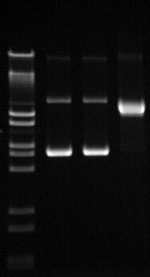
\includegraphics[width = 0.25\linewidth]{electro}
			\caption{Resultados de una electroforesis. En la imagen se pueden observar los resultados obtenidos para una electroforesis realizada para tres muestras diferentes, donde el pozo de la izquierda representa el marcador de peso.}
			\label{fig:0}
		\end{figure}
	
		\subsection{Purificaci\'on}
			Este proceso se lleva a cabo con el fin de eliminar posibles impurezas o reactivos que puedan interferir con la secuenciación, como lo son los primers, dNTPs, el MgCl$_2$ y la Taq Polimerasa. Para ello, existen varios kits de purificación comerciales que son ampliamente usados a nivel industrial. En este caso se propone la utilización del kit \textit{Wizard SV gel and PCR Clean-up System}, puesto que este permite recuperar hasta un 89 \% de un producto de 5000 bp aproximadamente \cite{kitBook}, debido a que hace uso de una membrana de afinidad al DNA; y se basa en el siguiente procedimiento:
			\begin{enumerate}
				\item Mezclar el Binding Buffer y el producto de la PCR en una relación 1:1 de 19.5 $\mu$L
				\item Transferir el producto a la columna e incubar por 1 min a temperatura ambiente
				\item Centrifugar a 14000 rpm/1min y descartar el contenido del eppendorf 
				\item Agregar 700 $\mu$L de \textit{Washing Buffer}
				\item Centrifugar a 14000 rpm/1min y descartar el contenido del eppendorf 
				\item Agregar 500 $\mu$L de \textit{Washing Buffer} y centrifugar por 5 min 
				\item Descartar contenido del eppendorf y centrifugar a 14000 rpm/2 min 
				\item Ensamblar la columna a un eppendorf de 1.5 mL
				\item Adicionar 30 $\mu$L de H$_2$O libre de nucleasas
				\item Incubar a temperatura ambiente por 1 minuto y centrifugar a 14000 rpm/1min 
				\item Descartar la columna y colocar el contenido del tubo eppendorf nuevo 0.1 mL
				\item Conservar a -20 $^\circ$C para secuenciar
			\end{enumerate}
			\begin{flushright}
				Procedimiento reportado por \citeauthor{kitBook}
			\end{flushright}
			
		\subsection{Secuenciaci\'on}
			Dado que el proyecto no tiene consideraciones presupuestales, se postula el uso de Illumina como método se secuenciaci\'on, dado su alta sensibilidad, profundidad y automatización, propio de un método de segunda generación. Lo anterior hace referencia a la alta eficiencia que ofrece Illumina, debido a que utiliza la tecnología de amplificación de PCR en puente, lo cual le permite disponer de muy poca cantidad de muestra y obtener una alta resolución en los resultados, dada la gran cantidad de reads obtenidos. 
			
			Por otro lado, para el procedimiento se propone el uso del kit \textit{MiniSeq High Output Kit}, ofrecido por \textit{BioSystems} \cite{MiniSeq}, puesto que este esta diseñado para re-secuenciación dirigida (\textit{targeted resequencing}), secuenciación de genomas pequeños, plásmidos y secuenciación de amplicones.
		
	\section{Selecci\'on del vector}
		Se propone la utilización de un plásmido como vector de clonación, puesto que estos tienen un bajo costo de producción y alta eficiencia de expresión puesto que permite la inserción del material genético de interés en una célula hospedera que produce el material recombinante a medida que se reproduce. Por lo anterior, se propone la utilización del plásmido \textit{pMONO-blasti-mcs}, ofrecido por \textit{InvivoGen} \cite{pMONO-blasti}, el cual es un pl\'asmido de clonación y expresión, puesto que este cuenta con un origen de replicación, un sitio de múltiple clonaje (MCS por sus siglas en inglés) y dos genes reporteros: un gen de resistencia al antibiótico \textit{Blasticidin-S} y uno para la degradación de lactosa \cite{izumi1991blasticidin}. Lo anterior con el fin de verificar, no  solo la correcta inserción del plásmido, sino la orientación del fragmento de interés en el mismo.
		
		\begin{figure}[h]
			\centering
			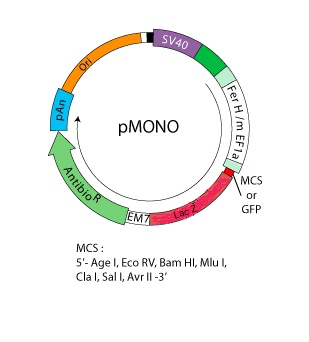
\includegraphics[width=0.5\linewidth]{plasmido}
			\caption{Pl\'asmido de expresión y clonación. En la figura se puede observar el diagrama representativo de la naturaleza del plásmido seleccionado. Es posible apreciar la ubicación del origen de replicación, los genes reporteros (Antibio R y Lac Z), el \textit{internal ribosome entry site} (IRES) y las posibles enzimas de restricción a utilizar}
			\label{fig:2}
		\end{figure}
	
		De la misma manera, se propone hacer uso de una cepa bacteriana de \textit{E. coli} no fermentadora de lactosa, puesto que se ha observado que esta tiene un alto nivel de producción, es exitosa en t\'erminos reproductivos, y está modificada para facilitar la verificación de la correcta inserción del vector de interés. Además, esta cepa es exitosa en el proceso de ''transferencia horizontal", por lo que tiene la capacidad de transferir el plásmido a otras células hospederas en el medio, bajo cierta presión de selección como la exposición a un antibiótico \cite{marraffini2008crispr}.
		
	\section{Seleccionar enzimas de restricci\'on}
		Como se puede observar en la \autoref{fig:2}, las posibles enzimas de restricción a utilizar para el plásmido seleccionado son Age I, EcoRV, BamHI, MluI, Cla I, Sal I y Avr II, por lo que se propone la utilización de la enzima BamHI, debido a que esta es de fácil obtención a nivel comercial y cuenta con dos sitios de restricción en el plásmido de interés, en la parte inicial y terminal del MCS respectivamente, según las indicaciones del proveedor. 
		
		Por otro lado, al realizar la digesti\'on del fragmento de interés por medio de la herramienta bioinformática \texttt{NEBcutter}, se obtuvieron los resultados de la \autoref{fig:3}.
		\begin{figure}[h]
			\centering
			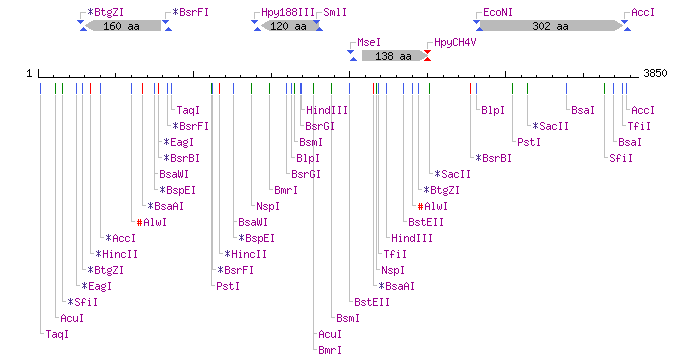
\includegraphics[width=\linewidth]{NEB0}
			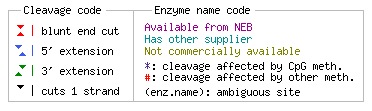
\includegraphics[width=0.6\linewidth]{NEB1}
			\caption{Resultados de la digestión enzimática por medio de la herramienta \texttt{NEBcutter}. En la figura se pueden observar los sitios de clivaje de las diferentes enzimas de restricción para el fragmento de interés y las convenciones de los mismos}
			\label{fig:3}
		\end{figure}
	
		Teniendo en cuenta los resultados observados en la \autoref{fig:3}, se propone la utilización de las enzimas ACC I, puesto que estas no solo cuentan con sitios de restricción en la zona de interés, evitando el clivaje del gen y de esta manera conservando la funcionalidad del mismo, sino que además no genera extremos romos en la secuencia, sino que al contrario, genera extremos cohesivos que facilitarán la inserción del fragmento en el vector de clonación.
		
	\section{Verificación de la transformación bacteriana}
		Para la inserción del fragmento de interés en el pl\'asmido seleccionado como vector de clonación se hace uso de una enzima DNA-Ligasa, en un medio acuoso libre de nucleasas y se realiza una electroforesis para comprobar la correcta inserción del fragmento de interés en el vector de clonación, de manera que se espera observar tres bandas de tamaño diferencial en el corrido electroforético. Una banda con un peso aproximado de 10 kb, que indica la inserción del fragmento de interés, otra con un tamaño de 7800 bp que indicaría el tamaño del plásmido sin el fragmento de interés, y una última de un tamaño aproximado de 7600-7700 kb que indicaría la digesti\'on enzimática, pero no introducción del fragmento de interés. Posteriormente, se realiza la transformación de la cepa bacteriana por medio de la técnica de electroporación, la cual es ampliamente usada en el ámbito de la biología molecular y consiste en la aplicación externa de un campo eléctrico al medio de cultivo que permite el aumento de la conductividad eléctrica y, de esta manera, un aumento de la permeabilidad de la membrana plasmática celular, creando de esta manera pequeños "poros'' en la misma, y permitiendo así la inserción del plásmido de interés en las células bacterianas.
		\subsection{Eficiencia reproductiva}
		Una vez introducido el vector de clonación en la cepa bacteriana, se debe realizar una siembra de la misma en un medio de cultivo de agar nutritivo con el fin de verificar el crecimiento de la cepa y, de esta manera confirmar que el vector no interfiere con ninguna de las rutas metabólicas determinantes para la viavilidad de la misma y determinar la eficiencia reproductiva y, asi mismo, el rendimiento relativo de la clonación del plásmido.
		
		\subsection{Confirmación de la introducción del plásmido en la cepa bacteriana}
		Una vez obtenida una alta densidad poblacional de la cepa, se realiza una segunda siembra de esta cepa viable a un medio suplementado con antibiótico Blasticidin-S con el fin de confirmar que el plásmido fue introducido a la bacteria. De esta manera, las cepas que tengan la capacidad de desarrollarse en este medio serán las que realmente hayan introducido el plásmido a su citoplasma. Además, el medio con el antibiótico tambien ejerce una presión de selección que favorece la transferencia horizontal entre organismos, promoviendo de esta manera una mayor producción del plásmido recombinante \cite{marraffini2008crispr}.
	
	\subsection{Verificación de la correcta inserción del fragmento de interés en el vector de clonación}
		Por último, el fragmento de interés podría haberse insertado en la dirección opuesta al marco de lectura de la polimerasa, por lo que no podría transcribir la proteína y, por ende, no podría expresarse. Es por esto que se eligió un plásmido con dos genes reporteros, puesto que el gen que permite la fermentación o utilización de la lactosa esta justo despu\'es del MCS, por lo que si este gen se expresa, implicaría que el fragmento recombinante ya fue leído de igual forma, en la misma dirección. Lo anterior implica entonces que si la bacteria es capaz de fermentar la lactosa habrá incluido el fragmento de interés en la dirección correcta del marco de lectura, por lo que las colonias de interés en este caso deberían lucir como la \autoref{fig:4} muestra a continuación en un medio diferencial como el caso de MacConkey \cite{harvey2007microbiology}.
		
		\begin{figure}[h]
			\centering
			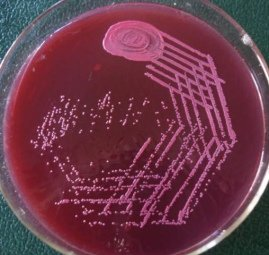
\includegraphics[width=0.4\linewidth]{mc}
			\caption{Colonias \textit{E. coli} lactosa positivo en agar MacConkey \cite{MacConkey}. La figura muestra como lucirían las colonias de interés en un medio selectivo y diferencial, suplementado con lactosa como fuente de carbono fermentable y antibiótico Blasticidin-S para evitar el crecimiento de flora acompañante.}
			\label{fig:4}
		\end{figure}

	\section{Extracción del plásmido recombinante}
		Habiendo confirmado la correcta inserción del fragmento de interés en el vector de clonación y el funcionamiento en la expresión del mismo, se desea realizar la extracción del plásmido recombinante con el fin de confirmar la correcta expresión y funcionalidad de la proteína de interés, para lo cuál se propone la utilización del kit \textit{Quantum Prep plasmid kit}, ofrecido por \textit{Bio-Rad} \cite{biorad}, para el cual se deben seguir los siguientes pasos:
		\begin{enumerate}
			\item Transferir 1.5 mL cultivo de \textit{E. coli} a un tubo  eppendorf, centrifugue por 1 min y descartar el sobrenadante
			\item Añadir 200 $\mu$L de la solución de resuspensión y resuspender el pellet con ayuda de una micropipeta
			\item Añadir 250 $\mu$L de la solución de lisis, mezclar por inversión 6 veces e incubar a temperatura ambiente por 5 min
			\item Añadir 250 $\mu$L de la solución de  neutralización. Mezclar por inversión 6 veces y centrifugar por 10 min a 13000 rpm
			\item Inserte la columna en un tubo eppendorf o de colección y adicione el sobrenadante de la mezcla a la columna
			\item Agregue 200 $\mu$L de \textit{Quantum Prep  matrix} a la columna. Mezcle por pipeteo. Centrifugue por 1 min a 13000 rpm y descarte el contenido del tubo 
			\item Añada 500 $\mu$L de Buffer de lavado y centrifugue por 1 min a 13000 rpm. (Repetir)
			\item Centrifugue por 2 min a 13000 rpm para  remover trazas de etanol
			\item Remueva la columna y pásela a un tubo limpio para luego añadir al centro de la columna 100 $\mu$L  de agua libre de nucleasas a 70 $^\circ$ C. Espere 1 minuto
			\item Centrifugue por 1 minuto a 13000 rpm y pase la columna a un tubo de recolección nuevo. Centrifugue por 1 minuto
			\item Almacenar a -20 $^\circ$C
		\end{enumerate}

		\begin{flushright}
			Procedimiento reportado por \citeauthor{bioradBook}
		\end{flushright}
	\section{Expresión de la proteína recombinante}
	
	La enzima Gliceraldehído-3-fosfato deshidrogenasa (GAPDH) cataliza una de las reacciones mas importantes en la ruta metabólica de la glucólisis a nivel celular, en la cual se forma bifosfoglicerato como producto y funciona como intermediario de alto contenido de energía, el cual en efecto es fundamental para la continuación de la ruta metabólica. Además, es durante este paso que tambi\'en se produce una molécula de NADH, que a su vez jugará un papel fundamental en la cadena de electrones para la producción de energía metabólica a nivel celular.
	
	Por lo anterior, se debe realizar una transformación de una cepa bacteriana de \textit{E. coli} modificada para la no expresión de la enzima GAPDH con el plásmido recombinante anteriormente extraído y, posteriormente, hacer una siembra en un medio de cultivo diferencial suplementado con glucosa como fuente de carbono fermentable con el fin de verificar la expresión y función de la proteína recombinante.
	
	\section{Extracción de la proteína recombinante}
	Con el fin de realizar un análisis estructural de la proteína de interés, se desea realizar la extracción y purificación de la misma a partir de la célula hospedera. Para esto, se hace uso de una cromatografía de afinidad con el fin de realizar el aislamiento de la proteína de interés y hacer lavados con un \textit{washing buffer} para finalmente realizar la elución de la proteína de interés a partir de la columna de afinidad. Esta técnica de separación hace uso de una fase móvil, como los buffers de lavado y elución, y una fase estacionaria compuesta por una columna de afinidad, en la cual se encuentra un ligando afín a la proteína de interés, por lo que se logra la retención de la misma hasta realizar la elución de ésta, por medio de un compuesto todavía mas afín al ligando anclado en la columna. De esta manera se puede obtener una solución de la proteína de interés únicamente.
	
	Por otro lado, otro método para extracción de la proteína involucra la extracción del proteoma completo del cultivo bacteriano que la expresa. Para esto se deben seguir los siguientes pasos:
	
	\begin{enumerate}
		\item Transferir 1000 $\mu$L del medio de cultivo con la cepa bacteriana y centrifugar 5 min a 13000 rpm
		\item Descartar 800 $\mu$L sobrenadante en hipoclorito y resuspender 
		\item Agregar el Buffer de muestra en una proporción 1:2 a 200 $\mu$L de muestra
		\item Calentar 100 $^\circ$C 5 min y centrifugar por 5 minutos a 13000 rpm 
		\item En el sobrenadante se encuentran las proteínas. Retirar el contenido viscoso del medio
	\end{enumerate}
	
	Adicionalmente, se propone la realización de un SDS-PAGE, el cual esta basado en un sistema electroforetico discontinuo, con el fin de lograr la separación de proteínas de interés. Para esto se debe preparar un gel de separación y otro de agrupamiento, realizando el siguiente procedimiento:
	
	\subsection{Preparación del gel de separación}
	\begin{enumerate}
		\item 2 mL solución de acrilamida
		\item 1.25 mL solución pH 8.8
		\item 1.75 mL H$_2$O
		\item Se debe adicionara además 50 $\mu$L de Persulfato de amonio (PA) y 8 $\mu$L de TEMED, los cuales corresponden al agente oxidante y reductor respectivamente y son factores fundamentales para la polimerización del gel
	\end{enumerate}
	
	\subsection{Preparación del gel de agrupamiento}
	\begin{enumerate}
		\item 325 $\mu$L soluci\'on acrilamida
		\item 625 $\mu$L soluci\'on pH 6.8
		\item 1.5 mL H$_2$O
		\item Agregar 30 $\mu$L de PA y 7 $\mu$L de TEMED
	\end{enumerate}
	
	Una vez realizado el montaje y preparados los geles, se procede con la adición del Buffer Tris-Glicina, la siembra de 8 mL de muestra y el marcador de peso, y el posterior corrido electroforético a 150 V por 90 min.
	
	\newpage
	\printbibliography[heading=bibintoc, title={Referencias}]
%	\bibliographystyle{plainnat}
\end{document}